%-------------------------------------------
\begin{frame}{
\includegraphics[height=0.8cm]{shared/logo-git.png}}
%-------------------------------------------
\begin{block}{Concepts, objects}
\begin{itemize}
    \item working directory: a user private copy of a whole repository of interest
    \item staging area: list of files of the working directory that will be considered for next commit (ie. could be not all the modified files)
    \item clone: a local copy of a repository (include all commits and branches), the original repository can be local, or remote (http access)
    \item commit: a git object, the snapshot of your entire repository compressed into a SHA (also the command the saves changes by creating the snapshot)
    \item HEAD: pointer representing your current working directory. Can be moved (git checkout) to different branches, tags, or commits 
    \item branch: a lightweight movable pointer to a commit
    \item merge: combines remote tracking branches into current local branch
\end{itemize}
\end{block}
\tiny{
   \url{https://www.tutorialspoint.com/git/git_quick_guide.htm}\\
   \url{https://www.powershellmagazine.com/2015/07/13/git-for-it-professionals-getting-started-2/}
}
\end{frame}

%-------------------------------------------
\begin{frame}[containsverbatim]
\frametitle{\raisebox{-1.5ex}{
\includegraphics[height=0.8cm]{shared/logo-git.png}} Setup}
%-------------------------------------------
\begin{block}{Git configuration: if not yet done, tell git our identity}
\begin{lstlisting}
git config --global user.name 'Your Name'
git config --global user.email 'Your Email'
\end{lstlisting}
\end{block}
\begin{block}{Git repository initialisation}
\begin{columns}
 \column{0.47\textwidth}
   The initialisation (red arrow) is the creation of a .git repository:
   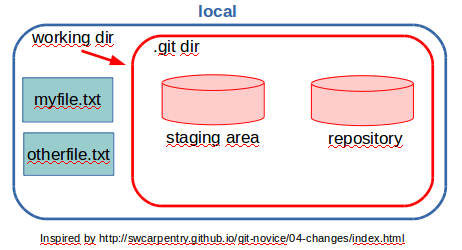
\includegraphics[height=3cm]{05_history/Images/FAIR_git_init.png}
    \column{0.52\textwidth}
   3 ways to initialize a .git repository:
   \begin{itemize}
       \item git init: inside an existing folder (possibly containing files)
       \item git init project: create the folder "project" + initializes the .git subfolder inside it
       \item git clone /gitfolder/path /new/path copy the existing git repository to a new one
    \end{itemize}
\end{columns}
\end{block}
\end{frame}
%-------------------------------------------
\begin{frame}[containsverbatim]
\frametitle{
\includegraphics[height=0.8cm]{shared/logo-git.png}}
%-------------------------------------------
\begin{block}{Tracking file}
\begin{columns}
 \column{0.5\textwidth}
git add command for myfile.txt:
 \begin{center}
   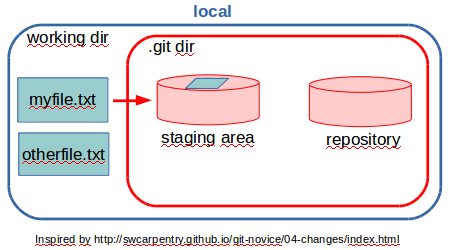
\includegraphics[height=3cm]{05_history/Images/FAIR_git_add.png}
\end{center}
 \column{0.5\textwidth}
git commit -m "my reason":
 \begin{center}
   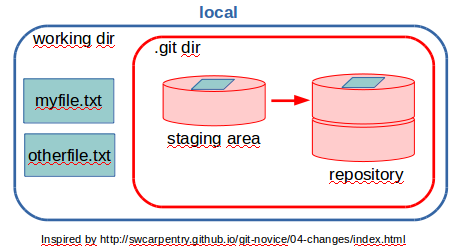
\includegraphics[height=3cm]{05_history/Images/FAIR_git_commit.png}
\end{center}
\end{columns}
\tiny{\url{http://swcarpentry.github.io/git-novice/fig/git-staging-area.svg}}
\end{block}
\begin{block}{Git file states}
Checking the file status: \verb|git status|\\
File goes from untracked to tracked state (init), unstaged to staged state (add) and finally, to a committed state (commit).
\end{block}
\end{frame}
%-------------------------------------------
%\begin{frame}{
\includegraphics[height=0.8cm]{shared/logo-git.png}}
%-------------------------------------------
%\begin{block}{File states and command}
%\begin{center}
%   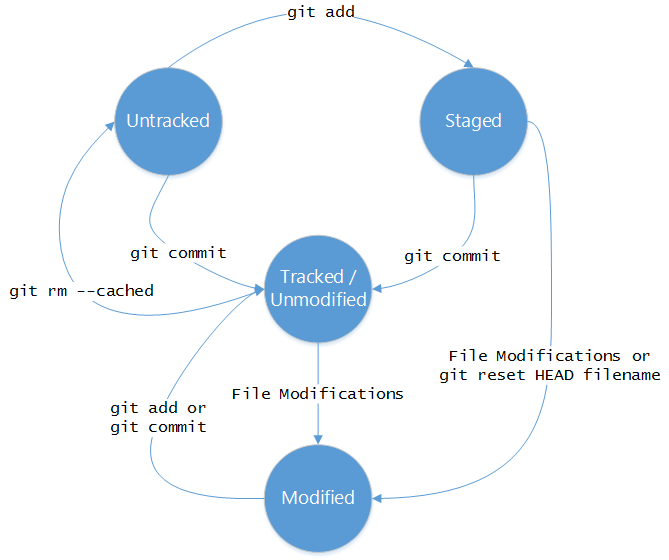
\includegraphics[height=6cm]{05_history/Images/FAIR_git_cycle.png}\\
%\tiny{\url{https://www.powershellmagazine.com/2015/07/13/git-for-it-professionals-getting-started-2/}}
%\end{center}
%\end{block}
%\end{frame}
